\chapter{Theoretical concepts}

Having talked about the MariX project and explained the motivation behind the development of a dual-color X-rays source, in this chapter I will explore the theoretical background needed to understand the experimental results obtained during the thesis work.
The first part of the chapter is dedicated to explaining the inverse Compton scattering process, while in the second broader part I will talk about optical resonators theory and its application to our Fabry-Perot cavities.

\section{The inverse Compton scattering process}
\subsection{Direct Compton and Thomson scattering}
Compton scattering was observed and explained by Arthur Holly Compton in 1923 \parencite{Compton1923}, the discovery earned him the 1927 Nobel Prize in Physics. The process consists in the scattering of a photon by a charged particle like an electron, in the interaction the static electron gains momentum while the photon loses energy and changes direction. The situation is represented in Fig \ref{fig:compton}. The effect was observed by sending X-rays against a graphite target, the published results demonstrated that light can't be fully described by a classical wave theory.
\begin{figure}
	\centering
	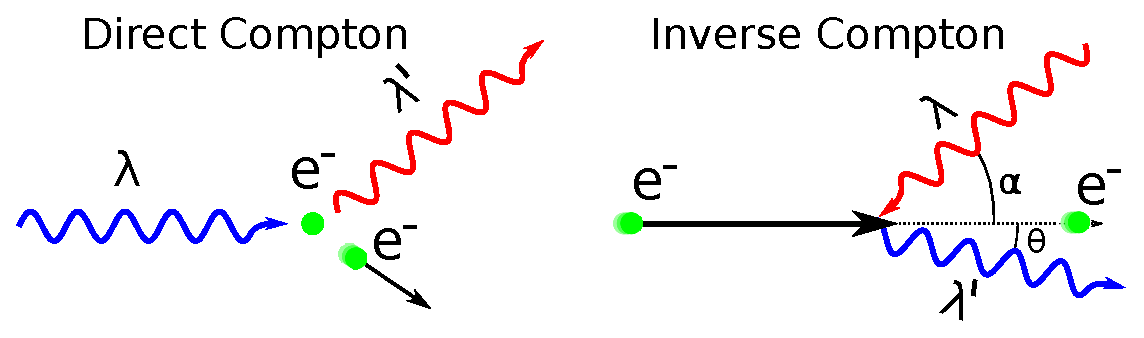
\includegraphics[width=0.9\linewidth]{images/compton.eps}
	\caption{On the left: Direct Compton scattering, the photon loses energy and the electron accelerates, the wavelength increases.
	On the right: Inverse Compton scattering, the photon recoils on the relativistic electron and gains energy proportional to the Lorentz factor squared $\gamma^2$, the wavelength decreases.}
	\label{fig:compton}
\end{figure}

In some occasions the interaction can be treated in the classical limit, in which case it is called Thomson scattering. Thomson scattering doesn't account for the change in wavelength of the incident light but represents a very good approximation when the photon frequency is low, in particular when $h\nu \ll m_e c^2$ is true.

We can describe the incident field as:
\begin{align}
\vec{E_i}= \hat{\epsilon} E_0 e^{i(\vec{k} \cdot \vec{x}-\omega t)}
\end{align}
where $ \hat{\epsilon}$ is the polarization versor. This field will displace the electron at position $\vec{x}_0$ by a small amount $\vec{x}(t) = \vec{x}_0+\delta \vec{x}(t)$. Using Newton's second law $\vec{F}=m \delta\ddot{\vec{x}}(t)$ we write:
\begin{align}
-e\,\hat{\epsilon} E_0 e^{i(\vec{k} \cdot \vec{x}-\omega t)} = m\delta\ddot{\vec{x}}(t)
\label{eq:newton}
\end{align}
In the Thomson limit we can use the approximation $\left|\delta\vec{x}\right| \ll \lambda$ to write $e^{i(\vec{k} \cdot \vec{x})} \approx e^{i(\vec{k} \cdot \vec{x}_0)}$. Solving then the differential equation \ref{eq:newton} yields
\begin{align}
\delta \vec{x}(t) = \frac{eE_0 e^{i(\vec{k} \cdot \vec{x}_0-\omega t)}}{m \omega^2} \hat{\epsilon}
\end{align}
The scattered light corresponds to the radiation emitted by the oscillating dipole $\vec{P}=-e\,\delta \vec{x}$, using the dipole emission formula \parencite{jackson_classical_1999} we can calculate the far field scattered emission at a distance $R$ from the source
\begin{equation}
\vec{E_s} = -\frac{k^2}{R} \,\hat{n} \times (\hat{n} \times \vec{P}) \,e^{ikR}
\end{equation}
The scattered light is polarized and has the same wavelength as the original light. An interesting quantity that can be calculated is the Thomson cross-section, which is $\sigma_T \approx 6.652 \times 10^{-29}\,\mathrm{m}^2$ (from \parencite{jackson_classical_1999}).

If the light is composed of high energy photons the classical approximation doesn't hold anymore, as the photons experience a change in wavelength due to the energy transfer with the electrons. In this case we need to describe light as comprised of photons with momentum
\begin{align}
\left|\vec{p_p}\right| = \frac{h\nu}{c} = \frac{h}{\lambda}
\end{align}
and energy
\begin{align}
E_p = p_p c = \frac{hc}{\lambda}
\end{align}
We consider a stationary electron, with energy equal to the rest energy $E_e = m c^2$ and momentum zero.
After the collision, the photon will have momentum  $\vec{p_p}'$ and energy $E_p'$.
Conservation of energy and momentum implies:
\begin{align}
E_p + m c^2 = E_p' + E_e' \\
\vec{p_p} = \vec{p_p}' + \vec{p_e}'
\end{align}
After some algebraic manipulation of these two equations, one obtains
\begin{align}
\frac{1}{p_f'}-\frac{1}{p_f} = \frac{1}{m c} \left( 1-\cos\theta\right)
\end{align}
where $\theta$ is the angle between $\vec{p_f}'$ and $\vec{p_f}$, that is the angle at which the photon is scattered. The Compton shift is then:
\begin{align}
\lambda'-\lambda = \frac{h}{m c} \left( 1-\cos\theta\right)
\end{align}
The maximum change in photon wavelength occurs when $\theta = 180\degree$, in this case the process is called Compton back-scattering.

\subsection{Inverse Compton scattering}
Direct Compton scattering deals with the case of a photon losing energy to an electron, when the opposite is true the process is called Inverse Compton Scattering. ICS occurs when photons are scattered by relativistic electrons ($v\sim c$), in this case the light is upshifted in frequency by a factor determined by the electrons velocity and proportional to $\gamma^2$, where $\gamma$ is the Lorentz factor. 
By making use of the principle of relativity we can describe the interaction in the electron rest frame and use the obtained results for direct Compton scattering, then return to the ``lab'' frame of reference using a Lorentz boost.

In the lab frame, the photon has frequency $\nu$ and is approaching the electron at an angle $\alpha$, the electron has relativistic velocity $\beta$, corresponding to the Lorentz factor $\gamma = 1/\sqrt{1-\beta^2}$. After the collision the photon will leave the interaction point at an angle $\theta$ with frequency $\nu_s$. The situation is represented in Fig \ref{fig:compton}.

We can calculate the photon frequency $\nu'$ in the electron rest frame using Lorentz transformations and remembering that $\vec{k} \cdot \vec{x}-\omega t$ is invariant under such transformations, we get:
\begin{align}
\nu' = \nu \gamma \left( 1+\beta \cos\alpha\right)
\end{align}
Since in BriXS the maximum energy reached by the electrons will be about 100\,MeV, corresponding to $\gamma \approx 200$, we can verify that in their rest frame the scattering occurs in the Thomson limit ($h \nu' \ll mc^2$):
\begin{align*}
h \nu' < 2 \gamma h \nu \approx 480\,eV && mc^2 \approx 5 \times 10^5\,eV
\end{align*}
In this limit the scattered light doesn't change frequency:
\begin{align}
\nu_s' = \nu'
\end{align}
but it changes direction, if we consider the light coming out at an angle $\theta'$ and then shift back to the lab frame via a second Lorentz boost we obtain:
\begin{align}
\nu_s = \nu_s' \gamma \left( 1-\beta \cos\theta'\right)
\end{align}
where
\begin{align}
\cos \theta' = \frac{\cos\theta -\beta}{1-\beta\cos\theta}
\end{align}
Substituting in the last expression we arrive at the final result, relating the scattering angles and the electron energy with the final photon energy:
\begin{align}
\nu_s = \nu\frac{1+\beta\cos\alpha}{1-\beta\cos\theta} \approx \nu\frac{2\gamma^2\left( 1+\cos\alpha\right)}{1+\gamma^2\theta^2}
\label{eq:ICS}
\end{align}
where the last approximation holds for $\theta\ll 1$. In practice, because of the second Lorentz boost, almost all the radiation is confined in an angle $\theta_m \approx 1/\gamma$ so the approximation is very accurate. Maximum emission and photon energy is reached for $\theta = 0$, varying the acceptance angle one can control the bandwidth of the extracted radiation \parencite{Drebot2017}, as showed in Fig \ref{fig:ics}.
\begin{figure}
	\centering
	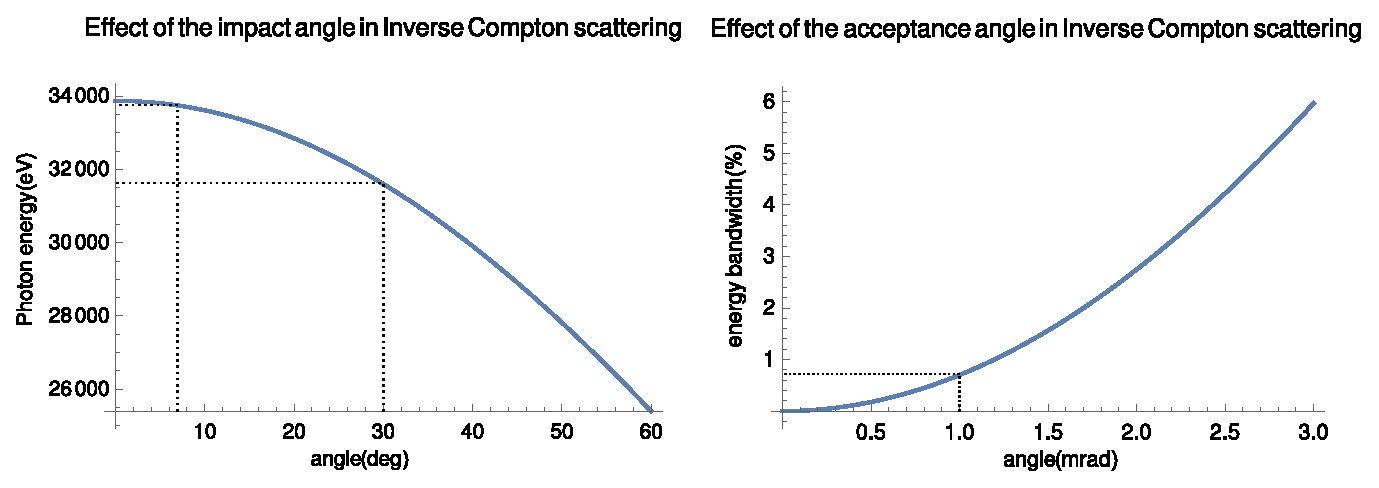
\includegraphics[width=1\linewidth]{images/ics.eps}
	\caption{Effect of the impact angle and of the acceptance angle in ICS: we can see that two cavities placed at $7\degree$ and $30\degree$ with respect to the electron beam produce the energies needed for iodine KES. BriXS will have a tunable bandwidth of $\Delta E/E \sim 1-10\%$, for KES the bandwidth must be kept low in order to achieve reasonable separation between the two colors, so a small acceptance angle ($\theta \approx 1$\,mrad) is preferred.}
	\label{fig:ics}
\end{figure}
Following \ref{eq:ICS} we can calculate the electron energy needed to reach the iodine K-edge, that is to produce X-rays with energy $h \nu_s \approx 34$\,keV in our first cavity. Given the geometry of the cavity and the mirror size the angle at the interaction point will be 7\degree, while
\begin{align}
\gamma = \sqrt{\frac{\nu_s}{\nu}\frac{1}{2(1+\cos 7 \degree)}} \approx 84
\end{align}
corresponding to an energy $E_e \approx$ 42\,Mev.
The second cavity will need to produce X-rays below the iodine edge, at 32\,keV. From the Fig \ref{fig:ics} we see that this is doable for an interaction angle of 30\degree. This means that the two crossed Fabry-Perot cavities will have to be placed with an angle of $23\degree$ between each other.

Different angles means also that the laser pulses interact with the electron bunches differently in the two cavity, in particular the time during which the pulses and the bunches overlap varies, this results in different luminosity for the two colors. Following \parencite{Variola2011} we can write the number of interaction per second in the Compton process as:
\begin{align}
N = \sigma_T f_\mathrm{rep} N_{ph} N_e G
\end{align}
where $G$ is the ``geometric factor'' and corresponds to the space-time interval in which the pulses and bunches overlap, $N_e$ and $N_{ph}$ are the electron and photon numerical densities, $f_\mathrm{rep}$ is the number of pulses interacting per second (equal to the repetition rate of the laser oscillator) and $\sigma_T$ the Thomson cross-section. Assuming a tri-gaussian shape for both, the rate of the scattering process is:
\begin{align}
N = \frac{\sigma_T f_\mathrm{rep} N_{ph} N_e}{2\pi\sqrt{\sigma_{Ly}^2+\sigma_{y}^2}\sqrt{\sigma_{Lx}^2+\sigma_{x}^2+\left(\sigma_{Lz}^2+\sigma_{z}^2\right)\tan^2(\frac{\alpha}{2})}}
\label{eq:N}
\end{align}
where the L subscript identifies the laser pulse dimensions as opposed to the electron bunch dimensions. To achieve the same luminosity for both the colors we can change the laser pulse dimension ($\sigma_{Ly}$ and $\sigma_{Lx}$) at the IP, compensating the $\sqrt{\tan^2(\alpha/2)}$ factor at the denominator.

Possible electron bunch and laser spot sizes are shown in Table \ref{tab:size}.
\begin{figure}
	\centering
	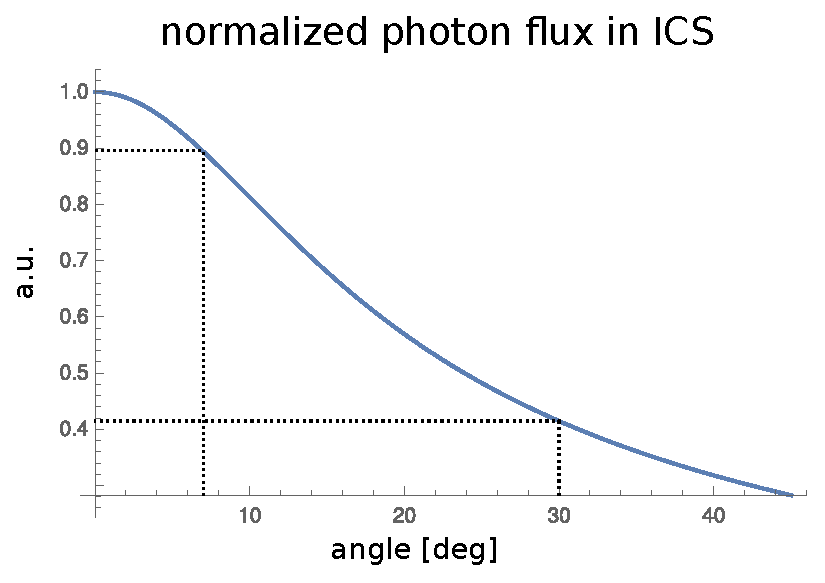
\includegraphics[width=0.9\linewidth]{images/photonflux.eps}
	\caption{Normalized photon flux in Inverse Compton Scattering as a function of the angle between the laser and the electron bunch. The values for the electron bunch and laser pulse size are that of the first two columns of \ref{tab:size}. Without changing the pulse size in the two cavities the flux would differ by a factor $\approx 2$.}
	\label{fig:photonflux}
\end{figure}
\begin{table}
	\centering
\begin{tabular}{|c|c|c|c|}
	\hline 
	&e$^- bunch$  &Laser $\alpha=7\degree$  &Laser $\alpha=30\degree$  \\ 
	\hline 
$\sigma_x [\mathrm{\mu m}] $	& 25 & 60 & 24 \\ 
	\hline 
$\sigma_y [\mathrm{\mu m}]$	& 15 & 40 & 15 \\ 
	\hline 
$\sigma_z [\mathrm{\mu m}]$  & 440 & 300 & 300 \\
	\hline

\end{tabular}
	\caption{Possible values for the electron bunches and laser pulses dimensions, this configuration gives the same luminosity for the two colors produced at different angles.}
\label{tab:size}
\end{table}

From \ref{eq:N}, and its dependence from the low Compton cross-section\\ ($\sigma_T=6.652\times 10^{-29}$\,m$^{-2}$) it is clear that a high photon flux is required to reach efficient generation of X-rays, hence the need for power enhancing Fabry-Perot optical cavities.

\section{Optical cavities}
\begin{figure}
	\centering
	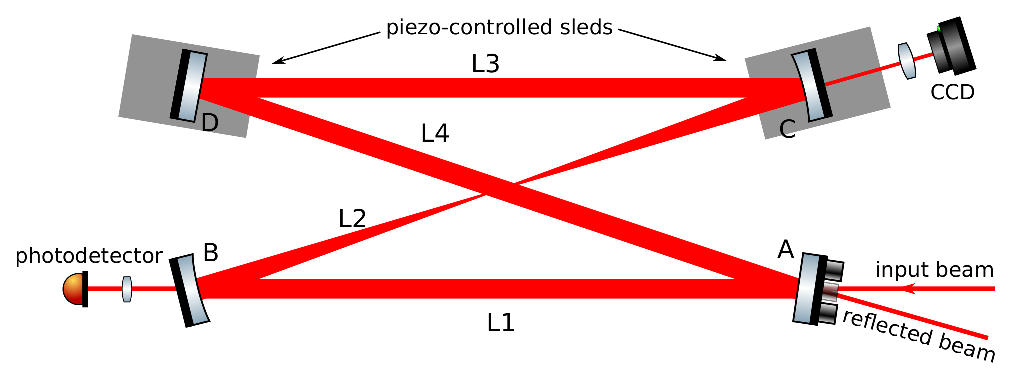
\includegraphics[width=1\linewidth]{images/cavity.eps}
	\caption{The 4-mirror confocal bow-tie cavity design. Mirror A is the input coupler and it is mounted on the piezoelectric ring crystal used by the PDH system to stabilize the cavity. B and C are the curved mirrors, they are mounted on a computer-controlled positioning system able to change their orientation, and in doing so move the cavity waist. Mirror C and D are mounted on two sleds used to adjust the cavity length, by moving both at the same time it is possible to change the distance between the curved mirrors while maintaining the cavity length. The reflected beam is used by the PDH system to create the error signal needed for the stabilization.}
	\label{fig:cavity}
\end{figure}

A resonant optical cavity consists of multiple optical elements that force light to travel in a closed path. The simplest such arrangement is two mirrors facing each other. A Fabry-Perot cavity is a passive optical resonator (i.e. without gain medium) in which only particular frequencies can be coupled (through an input coupler) and transmitted through the other mirrors, while other frequencies are reflected.
The optical power in the resonator is enhanced by a factor that depends on the cavity losses and the input coupling efficiency, those are determined mainly by the cavity mirrors reflectivity.

The proposed cavity design for BriXS, and the one developed in our laboratory, is a 4-mirror confocal bow-tie cavity. As we will see, a confocal cavity is very stable against the misalignment of optical elements, this is useful since our objective is to move the cavity focus in and out of the interaction point by deliberately misaligning the curved mirrors in the vertical direction, and in doing that we don't want to change the coupling with the external laser source or the resonating frequency. The cavity design is represented in Fig \ref{fig:cavity}.

\subsection{Ray optics and the ABCD matrix formalism}

To better understand the propagation of light waves inside a resonator we start by introducing the ABCD matrix formalism for optical ray propagation \parencite{Brouwer1964,siegman86}. We will also use this theoretical tool to make predictions on the behavior of the laser beam and waist inside the cavity.
\begin{figure}
	\centering
	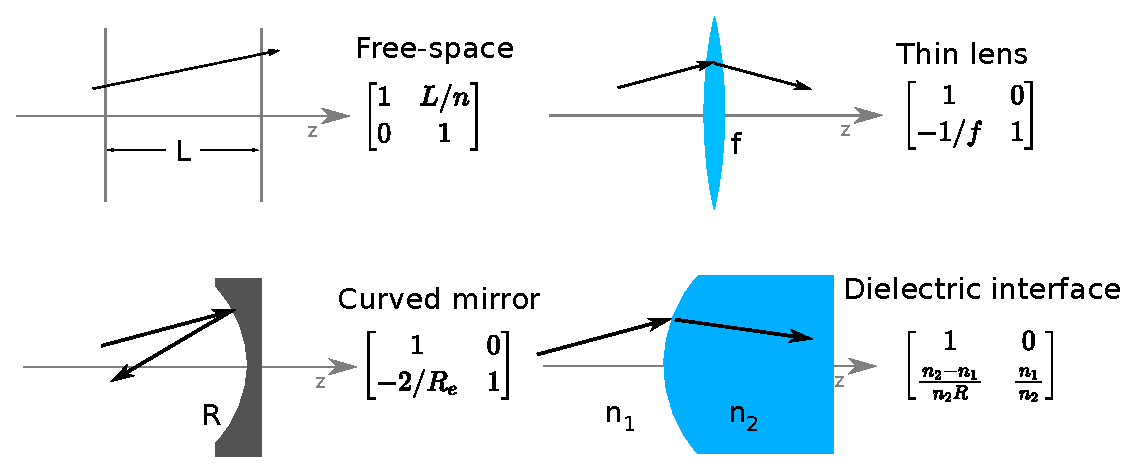
\includegraphics[width=1\linewidth]{images/abcd.eps}
	\caption{ABCD matrices for various paraxial optical elements. In the case of the curved mirror, $R_e$ is the ``effective radius'' for non normal incidence, equal to $R/\cos\theta$ for the vertical direction and $R\cos\theta$ in the horizontal direction, where $\theta$ is the angle of incidence. A curved mirror is an astigmatic element.}
	\label{fig:abcd}
\end{figure}

Let's consider a light ray traveling roughly in the $z$ direction, at a distance $r(z)$ from the reference $z$ axis and with a small inclination $r'=dr/dz$: if it travels from  location $z_1$ to $z_2$ for a length $L$, the distance and inclination $r_2$ and $r'_2$ in $z_2$ will be:
\begin{align}
r_2 &= r_1 + \frac{L}{n}\frac{dr_1}{dz} = r_1 + \frac{L}{n}r'_1  \\
r'_2 &= \frac{dr_2}{dz} = r'_1
\end{align}
where $n$ is the refractive index of the medium.
If the ray goes through a converging thin lens with focal distance $f$, its $r$ and $r'$ parameters immediately before and after the lens will be related by:
\begin{align}
r_2 &= r_1 \\
r'_2 &= -\frac{1}{f}r_1 +r'_1
\end{align}
Obviously the ray does not change its distance from the optical axis, but the slope changes because of the lens focusing power.
In both these cases a linear transformation relates the properties of the ray before the optical elements with that of the ray after the element. These transformations can then be written in matrix form, with the matrix acting on the ray vector $\boldsymbol{r} = (r,r')^T$:
\begin{align}
\begin{bmatrix}
	r_2 \\
	r'_2
\end{bmatrix}
=
\begin{bmatrix}
	A & B\\
	C & D
\end{bmatrix}
\begin{bmatrix}
	r_1 \\
	r'_1
\end{bmatrix}
\end{align}
The transformation representing the thin lens for example is:
\begin{align*}
\begin{bmatrix}
r_2 \\
r'_2
\end{bmatrix}
=
\begin{bmatrix}
1 & 0\\
-1/f & 1
\end{bmatrix}
\begin{bmatrix}
r_1 \\
r'_1
\end{bmatrix}
\end{align*}
Matrices representing other paraxial optical elements are shown in Fig \ref{fig:abcd}. It is important to note that the determinant of these ABCD matrix is given by $AB-CD=n_1/n_2$, or 1 in the case of the same medium. A complex system composed of multiple optical elements $M_1,M_2,\dots$ can then be described by a single ABCD matrix obtained by matrix multiplication:
\begin{align*}
M = \dots M_3 M_2 M_1
\end{align*}
By the property of matrix multiplication, $M$ will also have unitary determinant (if the ray starts and arrives in the same medium). A consequence of this fact is that every complex ABCD system between two optical planes can be described as a thin lens ($f$) surrounded by two free space propagations ($L_1$,$L_2$): since the matrix has only three free parameters, by accurately choosing $f,L_1,L_2$ one can recreate the same ABCD values of the complex system.
\begin{figure}
	\centering
	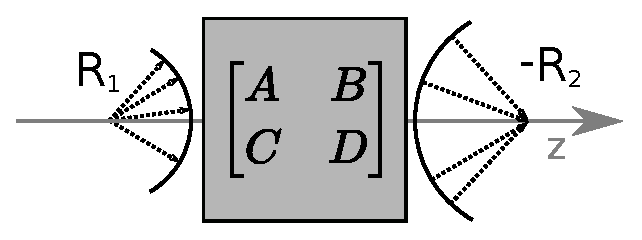
\includegraphics[width=0.9\linewidth]{images/abcdradius.eps}
	\caption{After passing through a general ABCD system, a spherical wavefront is still spherical but the radius of curvature is changed according to \ref{eq:radius}}
	\label{fig:radius}
\end{figure}

Ray matrices can also be used to describe the propagation of spherical waves: a spherical wave can be seen as a collection of rays originating from a common point but with different orientation, as shown in Fig \ref{fig:radius}. For each of these rays holds that:
\begin{align}
	r'(z) = \frac{dr}{dz} = \frac{r(z)}{R(z)}
\end{align}
where $R(z)$ is the distance from the wavefront center of curvature.
After passing through an ABCD system the wavefront radius will change following:
\begin{align}
R_2 = \frac{r_2}{r'_2} = \frac{Ar_1+Br'_1}{Cr_1+Dr'_1}= \frac{AR_1+B}{CR_1+D}
\label{eq:radius}
\end{align}
Thus, a spherical wavefront remains spherical after propagating through a paraxial optical system.

In 3D space a ray will in general be described by two displacements from the $z$ axis, in directions $x$ and $y$, if the ray passes through astigmatic elements, such as spherical mirrors with non-normal incidence, the matrices for the two directions will be different.

\subsubsection{Stability of optical resonators}
In an optical cavity the beam passes through the same optical elements (usually mirrors) over and over, if $M$ is the matrix representing the cavity, after $n$ passes the original ray $\boldmath{r_1}$ will become:
\begin{align}
\boldsymbol{r_2} = M^n \boldsymbol{r_1}
\end{align}
After an infinite number of passes the ray will either remain confined in a bounded region or diverge to infinity, in the first case the cavity is called stable, while in the other unstable.
We can study this behavior by expanding a generic ray on the cavity eigenrays, that is $\boldsymbol{r_{a,b}}$ such that:
\begin{align}
M \boldsymbol{r_{a,b}} = \lambda_{a,b} \boldsymbol{r_{a,b}}
\end{align}
A generic ray $\boldsymbol{r} = a \boldsymbol{r_{a}} + b \boldsymbol{r_{b}}$ will then evolve following:
\begin{align}
M^n \boldsymbol{r} = a \lambda_{a}^n \boldsymbol{r_{a}} + a \lambda_{b}^n \boldsymbol{r_{b}}
\end{align}
The eigenvalues can be found from $M$ via:
\begin{align}
	\begin{vmatrix}
	A-\lambda & B\\
	C & D-\lambda\\
	\end{vmatrix}
	&= \lambda^2 - (A+D)\lambda +1 = 0 \\
	\lambda_{a,b} &= m \pm \sqrt{m^2-1}
\end{align}
where $m=(A+D)/2$ is the so-called ``stability parameter'' (or ``m parameter'') for the system.
We can now see that if $-1\le m\le1$ then the two eigenvalues will be unitary conjugate complex numbers $e^{\pm i\theta}$, giving
\begin{align}
M^n \boldsymbol{r} = a e^{i\theta n} \boldsymbol{r_{a}} + b e^{-i\theta n} \boldsymbol{r_{b}} = \boldsymbol{s_1} \cos\theta n + \boldsymbol{s_2} \sin\theta n
\end{align}
The ray will remain confined in an area determined by the initial condition, the cavity in this case is stable.
If $|m|>1$ the two eigenvalues will be real and the ray will evolve according to:
\begin{align}
	M^n \boldsymbol{r} = \boldsymbol{s_1} \cosh\theta n + \boldsymbol{s_2} \sinh\theta n
\end{align} 
meaning that its propagation is unbound, the cavity is unstable.
\begin{figure}
	\centering
	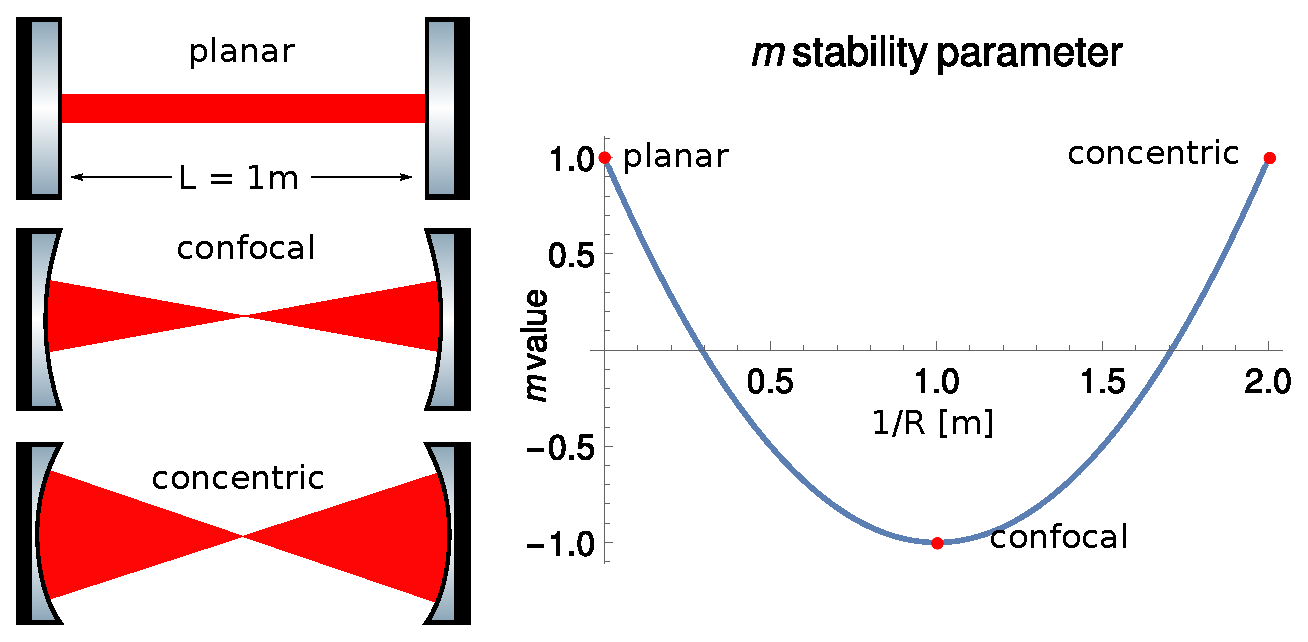
\includegraphics[width=1\linewidth]{images/mstability.eps}
	\caption{Three type of resonators: the planar and concentric cavities have $m=1$ while the confocal cavity has $m=-1$, they all are on the edge of stability. From the plot it is clear that a near-confocal cavity is stable while a near-concentric or near-confocal can have $m>1$.}
	\label{fig:mstability}
\end{figure}

Having explained the importance of the stability parameter, let's use it to determine the stability of various cavity types. In Fig \ref{fig:mstability} three different cavities composed by two curved mirrors are represented, their ABCD matrix representation can be obtained multiplying the matrices for the two mirrors and two free space propagations. We are interested in the stability parameter, if $R_1$ and $R_2$ are the radii of the mirrors and $L$ the distance between them $m$ is:
\begin{equation}
m = 2\left( 1- \frac{L}{R_1} \right)\left( 1- \frac{L}{R_2} \right)-1
\end{equation}
We can see in Fig \ref{fig:mstability} that confocal, concentric and planar resonators are on the ``stability edge''; however, small deviations in $L$, $R1$ or $R2$ can make a concentric or planar resonator unstable, while a confocal resonator remains stable.

\subsubsection{The 3x3 Matrix formalism for misaligned elements}

Until now we have considered optical elements perfectly placed and oriented on an imaginary optical axis, from which the ray parameters $r$ and $r'$ are calculated.
We can now study how a misaligned optical element acts on a light ray. A misaligned optical element acts with the same ABCD matrix but on an axis (called ``element axis'') different from the reference optical axis. The situation is represented in Fig \ref{fig:misaligned}.
\begin{figure}
	\centering
	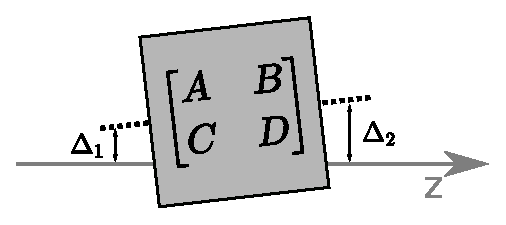
\includegraphics[width=1\linewidth]{images/misaligned.eps}
	\caption{A misaligned optical element: its axis does not match the reference optical axis $z$.}
	\label{fig:misaligned}
\end{figure}
Let's consider an optical ABCD element of length $L$ shifted by $\Delta_1$ from the optical axis at the input plane and $\Delta_2$ at the output plane, its slope in respect to the reference is 
\begin{align}
\Delta' = \frac{\Delta_2-\Delta_1}{L}
\label{eq:delta}
\end{align}
Assuming no changes happen in the refractive index, the slope is the same at the input and output planes.
The \ref{eq:delta} can also be written
\begin{align}
\boldsymbol{\Delta_2}=
\begin{bmatrix}
\Delta_2 \\
\Delta'
\end{bmatrix}
=
\begin{bmatrix}
1 & L \\
0 & 1 \\
\end{bmatrix}
\begin{bmatrix}
\Delta_1 \\
\Delta'
\end{bmatrix}
=M_\Delta \boldsymbol{\Delta_1}
\end{align}

A ray characterized by parameters $r_1$ and $r'_1$ will be represented on the element axis by
\begin{align}
s_1 = r_1 - \Delta_1 && s'_1 = r'_1 - \Delta'
\end{align}
We know how the element acts on $\boldsymbol{s_1}$:
\begin{align}
\boldsymbol{s_2} =
\begin{bmatrix}
s_2 \\
s'_2
\end{bmatrix}
=
\begin{bmatrix}
A & B \\
C & D \\
\end{bmatrix}
\begin{bmatrix}
s_1 \\
s_1'
\end{bmatrix}
=M \boldsymbol{s_1}
\end{align}
Returning to the reference axis we get the overall effect of the misaligned element:
\begin{align}
\boldsymbol{r_2} &= \boldsymbol{s_2} + \boldsymbol{\Delta_2}\\
\boldsymbol{r_2} = M\boldsymbol{s_1} + M_\Delta \boldsymbol{\Delta_1} &= M\boldsymbol{r_1} + (M_\Delta - M)\boldsymbol{\Delta_1} = M\boldsymbol{r_1} + \boldsymbol{E}
\end{align}
The misaligned element acts like its aligned counterpart except for the addition of an ``error vector'' $\boldsymbol{E}$ to the optical ray.
The total transformation $M\boldsymbol{r_1}+\boldsymbol{E}$ can be represented on a 3x3 matrix:
\begin{align}
\begin{bmatrix}
r_2 \\
r'_2 \\
1
\end{bmatrix}
=
\begin{bmatrix}
A & B & E\\
C & D & F\\
0 & 0 & 1
\end{bmatrix}
\begin{bmatrix}
r_1 \\
r_1'\\
1
\end{bmatrix}
\label{eq:abcdef}
\end{align}
\begin{align}
E = (1-A)\Delta_1 + (L-B)\Delta' && F = -C\Delta_1 + (1-D)\Delta'
\end{align}
This representation is very useful because it permits to easily calculate the overall matrix of a complex system of misaligned elements, such as a cavity with misaligned mirrors, via matrix multiplication.

If we consider a resonator and its ABCDEF round-trip matrix we can see that a ray lying on the reference optical axis $\boldsymbol{r} = (0,0,1)^T$ will in general not superimpose with itself after a round-trip of the cavity:
\begin{align}
\begin{bmatrix}
A & B & E\\
C & D & F\\
0 & 0 & 1
\end{bmatrix}
\begin{bmatrix}
0 \\
0\\
1
\end{bmatrix}
=
\begin{bmatrix}
E \\
F \\
1
\end{bmatrix}
\end{align}
To find the overall ``axis ray'' of the cavity, that is the ray that after a round-trip of the cavity has the exact same position and slope, one must solve the ``eigenray'' problem:
\begin{align}
M \boldsymbol{r_0} = \boldsymbol{r_0}
\end{align}
The solution is:
\begin{align}
r_0 = \frac{(1-D)E + BF}{2-A-D} && r_0' = \frac{CE + (1-A)F}{2-A-D}
\label{eq:eigenray}
\end{align}
This is the resonating ray of the cavity, all other rays will behave according to the results of the previous section on stable and unstable resonators in reference to this axis ray. In particular a ray $\boldsymbol{r_1}$ after a round-trip will evolve following:
\begin{align}
\boldsymbol{r_2}-\boldsymbol{r_0} = M_{2\times2} (\boldsymbol{r_1}-\boldsymbol{r_0})
\end{align}
To efficiently couple a Fabry-Perot cavity with an external ray, matching between the external ray and the axis ray is required.
It is important to note that for a near planar or near concentric cavity $A+D \approx 2$, according to \ref{eq:eigenray} this means that the cavity is extremely unstable regarding misalignment, while for a near confocal cavity $A+D \approx -2$ giving maximum stability.

\subsubsection{Cavity focus movement through moving mirrors}
We can now apply this formalism to our crossed cavities and verify that we can move the ray resonating in the cavity, and in particular the location of the beam waist between the curved mirrors, by accurately tilting the curved mirrors.

Since the objective is to use this movement to vertically move the focus of one cavity in and out of the interaction point with the electrons, we need to calculate the round-trip matrix for the vertical direction. The ABCDEF matrix for the plane mirrors is simply the identity matrix\footnote{We don't consider ray inversion\parencite{siegman86,Plachenov2011} since our cavity has an even number of mirrors.}, while that of the tilting curved mirrors is :
\begin{align}
M_{b,c}(d\alpha) = 
\begin{bmatrix}
1 & 0 & 0\\
-2\frac{\cos\theta/2}{R_{b,c}} & 1 & 2d\alpha\\
0 & 0 & 1
\end{bmatrix}
\end{align} 
where $d\alpha$ is the tilt angle, $\theta/2$ the angle of incidence on the mirror and $R_{b,c}$ the mirror radius of curvature (in our case $\theta/2 = 7\degree /2 = 3.5\degree$ and $R_b=R_c=750$\,mm).
The free space propagation matrix has the expression:
\begin{align}
M_L = 
\begin{bmatrix}
1 & L & 0\\
0 & 1 & 0\\
0 & 0 & 1
\end{bmatrix}
\end{align}
The overall cavity matrix calculated from the focus plane is then:
\begin{align}
\begin{split}
M = 
\begin{bmatrix}
1 & L_2/2 & 0\\
0 & 1 & 0\\
0 & 0 & 1
\end{bmatrix}
\begin{bmatrix}
1 & 0 & 0\\
-2\frac{\cos\theta/2}{R_{b}} & 1 & 2d\alpha\\
0 & 0 & 1
\end{bmatrix}
\begin{bmatrix}
1 & L_1 & 0\\
0 & 1 & 0\\
0 & 0 & 1
\end{bmatrix}
\begin{bmatrix}
1 & L_4 & 0\\
0 & 1 & 0\\
0 & 0 & 1
\end{bmatrix}\\
\begin{bmatrix}
1 & L_3 & 0\\
0 & 1 & 0\\
0 & 0 & 1
\end{bmatrix}
\begin{bmatrix}
1 & 0 & 0\\
-2\frac{\cos\theta/2}{R_{c}} & 1 & 2d\alpha\\
0 & 0 & 1
\end{bmatrix}
\begin{bmatrix}
1 & L_2/2 & 0\\
0 & 1 & 0\\
0 & 0 & 1
\end{bmatrix}
\end{split}
\end{align}
\begin{figure}
	\centering
	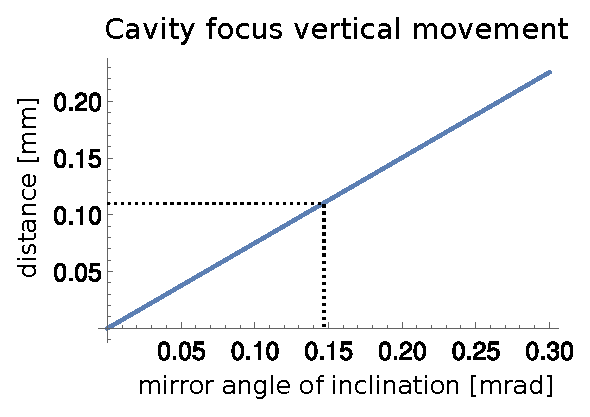
\includegraphics[width=0.8\linewidth]{images/shiftfocus.eps}
	\caption{Focus vertical movement versus angular misalignment of mirrors B and C, to reach $110\,\mu$m of movement we need to tilt the mirrors for about $150\,\mu$rad.}
	\label{fig:shiftfocus}
\end{figure}
where the lengths $L_i$ are distances between the mirrors labeled in Fig \ref{fig:cavity}. 
The focus vertical movement $r_0(d\alpha)$ is then given by \ref{eq:eigenray}, the results are shown in Fig \ref{fig:shiftfocus}.
If we consider the possible spot sizes given in Tab \ref{tab:size} we can see that to switch between the two cavities we need a movement of at least $w_{1y}+w_{2y}=2(\sigma_{1y}+\sigma_{2y})\approx 110\,\mu$m, corresponding to a mirror inclination of about $150\,\mu$rad.

The cavity length is unaffected by the mirror movement if the rotation pivot is at the same height as the laser beam. However our mirrors rotate around an axis situated about $r =16$\,mm under the laser beam height, that means that during the rotation the mirror moves forward. The cavity length would be reduced by
\begin{align}
	\delta L = \frac{4 r d\alpha }{\cos 3.5\degree}
\end{align}
which amounts to about $10\,\mu$m for the desired movement, just beyond the limit of our current stabilization system. To eliminate this problem, new mirror mounting with gimbal-like movement are being developed in our laboratory.

\subsection{Longitudinal and transverse modes}

Light propagation inside a cavity can be described using Huygens integral, considering each point as a spherical wave source, and the paraxial approximation. Given an electric field distribution $E_0(x_0,y_0,z_0)$ (we assume sinusoidal time dependence) Huygens integral allows us to calculate the field in a generic point via:
\begin{align}
\begin{split}
&E(x,y,z) =\\ &\frac{i}{\lambda}\frac{e^{-ik(z-z_0)}}{z-z_0}\iint E_0(x_0,y_0,z_0) \exp\left[-ik\frac{(x-x_0)^2+(y-y_0)^2}{2(z-z_0)}\right]\mathop{dx_0}\mathop{dy_0}
\end{split}
\label{eq:huygens}
\end{align}
where $(z-z_0)^2\gg(x-x_0)^2+(y-y_0)^2$ for the validity of the paraxial (or ``Fresnel'') approximation.
This is true for free-space propagation, however if the field goes through an ABCD optical system (like an optical cavity) eq. \ref{eq:huygens} becomes \parencite{svelto2010}:
\begin{align}
\begin{split}
&E(x,y,z) =\\ &\frac{i}{\lambda}\frac{e^{-ikB}}{B}\iint E_0 \exp\left[-ik\frac{A(x_0^2+y_0^2)+D(x^2+y^2)-2(xx_0+yy_0)}{2B}\right]\mathop{dx_0}\mathop{dy_0}
\end{split}
\label{eq:huy2}
\end{align}
By substitution it can be verified that functions of the form:
\begin{align}
f_0(x,y) \propto \exp\left[-ik\frac{x^2+y^2}{2q_0}\right]
\label{eq:gauss}
\end{align}
where $q_0$ is a complex parameter (we ignored the longitudinal phase-shift $\exp -ik(z-z_0)$\,), are ``eigensolutions'' of \ref{eq:huy2}, if substituted in the integral one gets:
\begin{align}
f(x,y) \propto \frac{1}{A+B/q_0} \exp\left[-ik\frac{x^2+y^2}{2q}\right]
\end{align}
where $q$ is given by:
\begin{align}
	q = \frac{Aq_0+B}{Cq_0+D}
	\label{eq:q}
\end{align}
A field described by \ref{eq:gauss} is called gaussian beam, while $q$ is called the complex beam parameter. The transformation of $q$ through an optical element is similar to that of the radius of spherical wavefront, in fact if $q$ is real the gaussian beam field becomes a spherical wave field. The imaginary part of $q$ gives the transverse width of the beam, this is clear by separating $1/q$ in its real and imaginary part:
\begin{align}
	\frac{1}{q} = \frac{1}{R} -i \frac{\lambda}{\pi w^2}
\end{align}
and substituting in the gaussian beam field expression
\begin{align}
f(x,y) \propto \exp\left[-\frac{x^2+y^2}{w^2}\right] \exp\left[-ik\frac{x^2+y^2}{2R}\right]
\end{align}

The gaussian beam is not the only eigensolution of the Huygens integral, other solutions are given by the Hermite-Gauss modes:
\begin{align}
HG_{nm}(x,y)  \propto H_n\left(\frac{\sqrt{2}x}{w}\right)H_m\left(\frac{\sqrt{2}y}{w}\right)\exp\left[-ik\frac{x^2+y^2}{2q}\right]
\label{eq:HG}
\end{align}
where $H_l$ are the Hermite polynomials. These modes are orthogonal to each other and form a complete system for the electric field, they also include the gaussian beam as the lowest order mode $HG_{00}$. In an astigmatic system $q_x$ and $q_y$ will in general be different.

For a mode $E_0$ to resonate in a cavity it is not enough to retain its transverse shape after a round trip, it must also return with the same phase, that means that the mode ``eigenvalue'' $\sigma$ given by:
\begin{align}
E_{rt}(x,y,z) = \sigma E_0(x,y,z)
\end{align}
must be real. This translates to a condition on the Hermite-Gauss mode frequencies inside the resonator \parencite{siegman86}:
\begin{align}
	\nu_{lmn} = \nu_{\mathrm{FSR}}\left(l+\frac{n+1/2}{2\pi}\arccos(m_H)+\frac{m+1/2}{2\pi}\arccos(m_V)\right) 
\end{align}
Where $m_H$ and $m_V$ are the two stability parameters for an astigmatic cavity.
The mode eigenvalue $\sigma$, in addition to determining if a mode is resonant, gives the diffraction power losses of the mode after a round-trip via:
\begin{align}
	\gamma = 1- |\sigma|^2
\end{align}
\begin{figure}
	\centering
	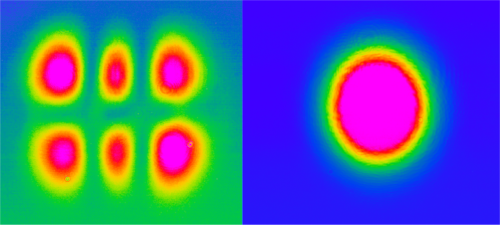
\includegraphics[width=1\linewidth]{images/modi.png}
	\caption{Two resonant modes observed in our cavity, in the left picture the $HG_{21}$ while in the right the fundamental mode $HG_{00}$.}
	\label{fig:modi}
\end{figure}

The $HG$ modes are only approximations (albeit good) of the modes inside a real resonator, real cavity modes are subject to diffractive effects (for example due to finite mirror size) and other non-idealities. An example of modes resonating in our Fabry-Perot cavities is shown in Fig \ref{fig:modi}, for our application (inverse Compton scattering) the cavities must be stabilized to resonate only with the lowest order $HG_{00}$ mode.

To excite a mode inside the cavity, mode matching between the laser external mode and the cavity is necessary. This means that the laser oscillator output must be single-mode ($HG_{00}$) and that the $q$ parameter must be controlled, this can be achieved by a telescopic system outside the cavity. The external mode must also lie on the ``axis ray'' of the cavity (defined in the previous section), however, during the curved mirror movement, the axis ray changes. The ray parallel shift is given by $r_0$ in \ref{eq:eigenray} (the change in the angle $r_0'$ is effectively 0). To estimate the change in coupling efficiency between the two modes we can then use the overlap integral of the modes at the input coupler:
\begin{align}
	\eta(r_0) = \int H_{00}^\mathrm{cav*}(x,y-r_0)H_{00}^\mathrm{ext}(x,y)\mathop{dx}\mathop{dy} 
	\label{eq:eta}
\end{align} 
The results shown in Fig \ref{fig:couplingeta} indicate that the change in coupling efficiency is very small ($<0.5\%$).
\begin{figure}
	\centering
	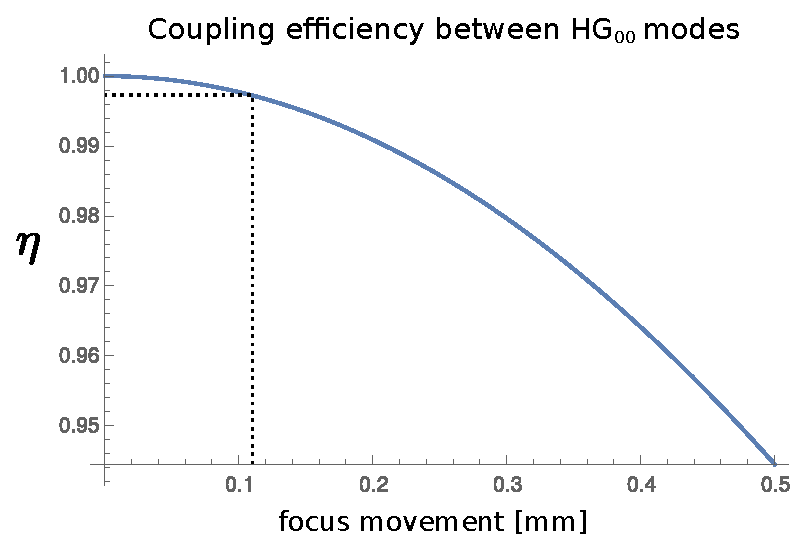
\includegraphics[width=0.8\linewidth]{images/couplingeta.eps}
	\caption{Coupling efficiency between two gaussian beams. The beam radius is set at $1.48\,$mm, as it is in our cavity. For a focus movement of $110\,\mu$m the efficiency remains over 99.5\%.}
	\label{fig:couplingeta}
\end{figure}

\subsection{Cavity Finesse and enhancement of the optical power}
\begin{figure}
	\centering
	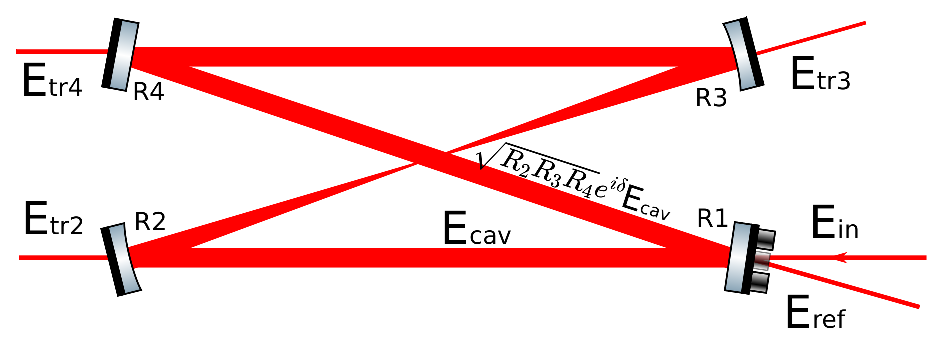
\includegraphics[width=0.9\linewidth]{images/ecav.eps}
	\caption{Electric fields inside the cavity. A full round trip of the cavity carries a phase factor $e^{i\delta}$ and a reflection on the input mirror causes a phase shift of $\pi$.}
	\label{fig:ecav}
\end{figure}
\begin{figure}
	\centering
	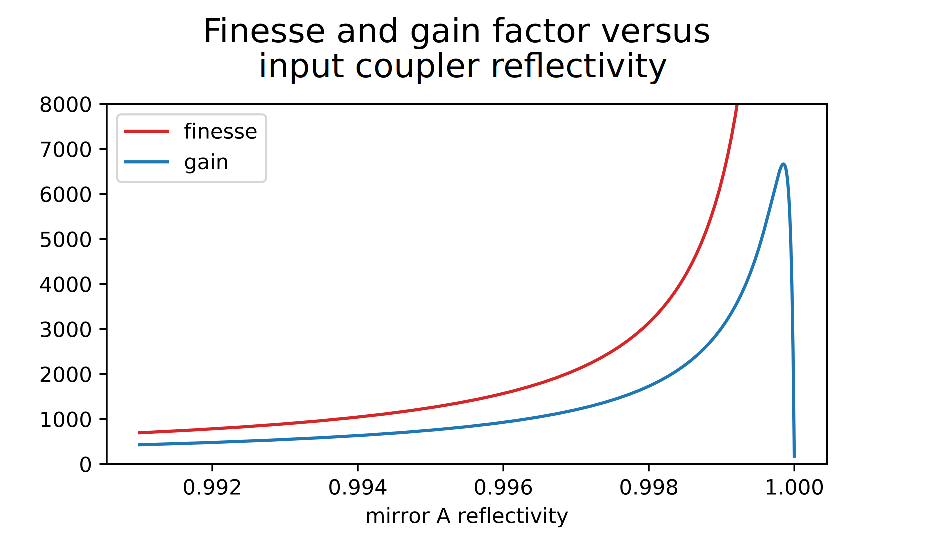
\includegraphics[width=0.9\linewidth]{images/finessegain.eps}
	\caption{Finesse and gain of a 4-mirror Fabry-Perot cavity. The reflectivities of mirror B, C and D are set to 0.99995. When the input coupler (mirror A) transmission is high the $a$ factor goes to $\pi/2$.}
	\label{fig:finessegain}
\end{figure}
\begin{figure}
	\centering
	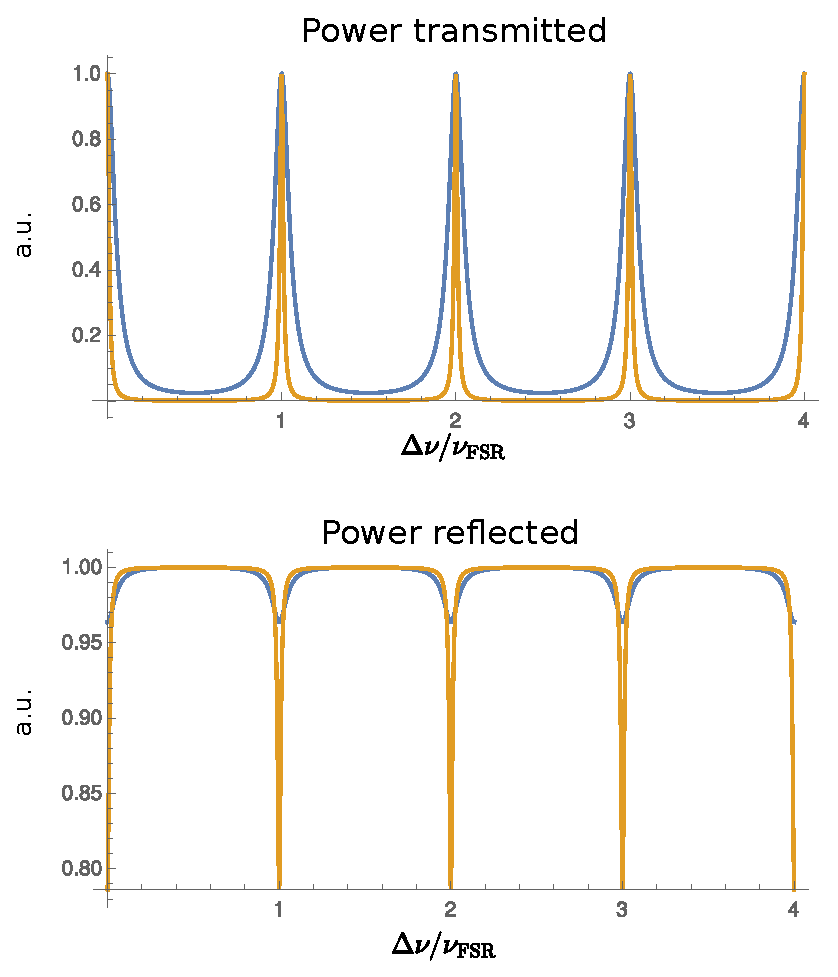
\includegraphics[width=0.9\linewidth]{images/reflected.eps}
	\caption{Transmission and reflection spectra of cavities with different Finesse (blue line for Finesse 10, orange for Finesse 50). The highest the Finesse the lowest the cavity bandwidth.}
	\label{fig:reflected}
\end{figure}

The field amplitude inside the Fabry-Perot cavity depends only on the mirror reflectivities. The field in a point inside the cavity must be equal to the sum of the same field after a round trip and the field that just entered the cavity through the first mirror, following Fig \ref{fig:ecav} we can write:
\begin{align}
	E_{\mathrm{cav}} &= \sqrt{1-R_1} E_{\mathrm{in}} +\sqrt{R_1R_2R_3R_4}e^{i\delta}E_{\mathrm{cav}} \\
	E_{\mathrm{cav}} &= \frac{\sqrt{1-R_1}}{1-\sqrt{R_1R_2R_3R_4}e^{i\delta}} E_{\mathrm{in}}
\end{align}
where $\delta=2\pi\Delta\nu/\nu_{\mathrm{FSR}}$ and $\Delta\nu=\nu-\nu_0$ is the ``detuning'' of the input frequency from the fundamental mode frequency.
From this we can derive the field transmitted through every mirror and the field reflected by the input coupler:
\begin{align}
E_{\mathrm{tr2}} &=  \sqrt{1-R_2}E_{\mathrm{cav}}\\
E_{\mathrm{tr3}} &=  \sqrt{(1-R_3)R_2}E_{\mathrm{cav}}\\
E_{\mathrm{tr4}} &=  \sqrt{(1-R_4)R_3R_2}E_{\mathrm{cav}}\\
E_{\mathrm{ref}} &=	 -\sqrt{R_1}E_{\mathrm{in}}+	\sqrt{(1-R_1)R_4R_3R_2}E_{\mathrm{cav}} \label{eq:ref}
\end{align}
The optical power inside the cavity will be given by $P_{\mathrm{cav}}\propto|E_{\mathrm{cav}}E_{\mathrm{cav}}^*|$ and the enhancement factor $P_{\mathrm{cav}}/P_{\mathrm{in}}$ can be calculated as:
\begin{align}
\frac {P_{\mathrm{cav}}}{P_{\mathrm{in}}} = \frac{1-R_1}{1+R-2\sqrt{R}\cos\delta}
\label{eq:power}
\end{align}
where $R=R_1R_2R_3R_4$.
Maximum power is reached for $\Delta\nu = n\nu_{\mathrm{FSR}}$, that is the resonance condition.

Another important property of a Fabry-Perot resonator is its Finesse, defined as the ratio between the free spectral range and the cavity linewidth. The cavity linewidth $\delta\nu$ can be found imposing $P_\mathrm{cav}(\delta\nu/2) = 1/2 P_\mathrm{cav}(0)$, a detuning of half linewidth reduce the power in the cavity by a factor of 2. This gives:
\begin{align}
\delta\nu = \nu_\mathrm{FSR} \frac{1-\sqrt{R}}{\pi R^{\frac{1}{4}}}
\end{align}
And so the Finesse is:
\begin{align}
	F = \frac{\nu_\mathrm{FSR}}{\delta\nu} = \frac{\pi R^{\frac{1}{4}}}{1-\sqrt{R}}
	\label{eq:finesse}
\end{align}
Transmission and reflection spectra of cavities with different Finesse are shown in Fig \ref{fig:reflected}.
The Finesse is related to the power gain of the cavity by
\begin{align}
	Gain = \frac{F}{a}
\end{align}
where $a$ is a numerical factor that tends to $\pi/2$ when the cavity losses are determined mainly by the input coupler transmission. Since $\pi/2$ is the minimum value assumed by $a$, this is the kind of cavity with maximum gain for a given Finesse, and the one used in BriXS. 

\subsection{Spectral coupling between cavity and oscillator}

To obtain maximum coupling between the cavity and the oscillator it is not enough to obtain spatial mode-matching (as described earlier by the overlap integral of Eq. \ref{eq:eta}), spectral matching between the two frequency combs must also be optimized.

\subsubsection{Effect of the $f_\mathrm{CEO}$}
The Carrier-Envelope-Offset (CEO) of the mode-locked laser (shown in Fig. \ref{fig:comb}) is a cause of mismatch between the spectral comb of the laser and that of the cavity.

The output field of a mode-locked laser can be described by the sum of the pulses:
\begin{align}
E(t) = \sum_{n} A(t-nt_r) e^{-i\omega_0 (t - nt_r)} e^{i \delta\Phi n}
\end{align}
where $A(t)$ is the pulse envelope, $\omega_0/2\pi$ is the carrier frequency, $t_r$ is the time between two successive pulses and $\delta\Phi$ is the CEO.
In the frequency domain it can be written (via Fourier transform):
\begin{align}
\tilde{E}(\omega) = \sum_n \tilde{B}(\omega) e^{i\omega n t_r} e^{i \delta\Phi n}
\end{align}
with $\tilde{B}(\omega)$ being the transform of $A(t) e^{-i\omega_0 t}$.
Because of the summation over $n$, the only frequencies $\omega_m$ that contribute are those that satisfy
\begin{align}
	\omega_m t_r + \delta \Phi = 2\pi m \\
	\omega_m = \frac{2\pi m}{t_r} -\frac{\delta \Phi}{t_r}
\end{align} 
Rewriting the last equation we get
\begin{align}
f_m = m f_\mathrm{rep} + f_\mathrm{CEO} && f_\mathrm{CEO} = -\frac{\delta \Phi}{2\pi t_r}
\end{align}
The cavity instead resonates at frequencies of the form:
\begin{align}
f_{cm} = m f_\mathrm{FSR}
\end{align}
with $f_\mathrm{FSR} = c/L$.
When the resonator and the oscillator are stabilized against each other we have that for a certain mode $m_0$ holds
\begin{align}
	m_0 f_\mathrm{rep} + f_\mathrm{CEO} = m_0 f_\mathrm{FSR}
\end{align}
In our cavity $m_0$ is about $L/\lambda_0=3\times10^6$. The relation doesn't hold for the other modes $m = m_0 +\delta m$, in fact the frequency mismatch between $f_m$ and $f_{cm}$ is given by 
\begin{align}
\Delta \nu &=  ((m_0+\delta m) f_\mathrm{rep} + f_\mathrm{CEO})-(m_0+\delta m)(f_\mathrm{rep} + f_\mathrm{CEO}/m_0)\\
\Delta \nu &= -f_\mathrm{CEO}\frac{\delta m}{m_0} = -f_\mathrm{CEO}\delta m\frac{\lambda_0}{L}
\end{align}
By writing the shift $\delta m $ in terms of a shift in wavelength
\begin{align}
	\delta m = \frac{\delta \nu}{f_\mathrm{rep}} = -\frac{c}{f_\mathrm{rep}\lambda_0^2}\delta\lambda
\end{align}
we finally get
\begin{align}
	\Delta \nu(\delta\lambda) = \frac{c f_\mathrm{CEO}}{f_\mathrm{rep}\lambda_0 L}\delta\lambda
\end{align}
$\Delta \nu$ is the difference between the laser mode frequency at $\lambda_0+\delta\lambda$ and the nearest cavity mode frequency.

An external mode will be coupled in the cavity only if $\Delta\nu(\delta\lambda)$ is within a cavity linewidth $\delta\nu_c$ from a cavity mode. The amount of modes coupled into the cavity depends on $f_\mathrm{CEO}$, i.e. the spectral coupling efficiency depends on $f_\mathrm{CEO}$. That means that if an incoming laser pulse has a spectrum of width $\Delta \lambda$:
\begin{align}
	S_\mathrm{in}(\delta\lambda) \propto \exp[-2 \frac{\delta\lambda^2}{\Delta\lambda^2}]
\end{align}
The pulse inside the cavity, and the pulse transmitted by the cavity, will have a spectrum:
\begin{align}
	S_\mathrm{out}(\delta\lambda) \propto S_\mathrm{in}(\delta\lambda)  \exp[-2\frac{\Delta\nu(\delta\lambda)^2}{\delta\nu_c^2}] 
\end{align}
The spectral coupling efficiency $\eta_\mathrm{sp}$ will then be given by the ratio of the two integrated spectra:
\begin{align}
	\eta_\mathrm{sp} = \frac{\int \exp[-2 \frac{\delta\lambda^2}{\Delta\lambda^2}]\exp[-2\frac{\Delta\nu(\delta\lambda)^2}{\delta\nu_c^2}]\,\mathrm{d}\delta\lambda}{\int \exp[-2 \frac{\delta\lambda^2}{\Delta\lambda^2}]\,\mathrm{d}\delta\lambda}
\end{align}

A plot of $\eta_\mathrm{sp}(f_\mathrm{CEO})$ is given in Fig \ref{fig:spectraleta} , we can see that to achieve bigger efficiency we can limit the spectrum entering the cavity, a feedback system to control the $f_\mathrm{CEO}$ (that depends on the temperature of the active medium) is also needed.
\begin{figure}
	\centering
	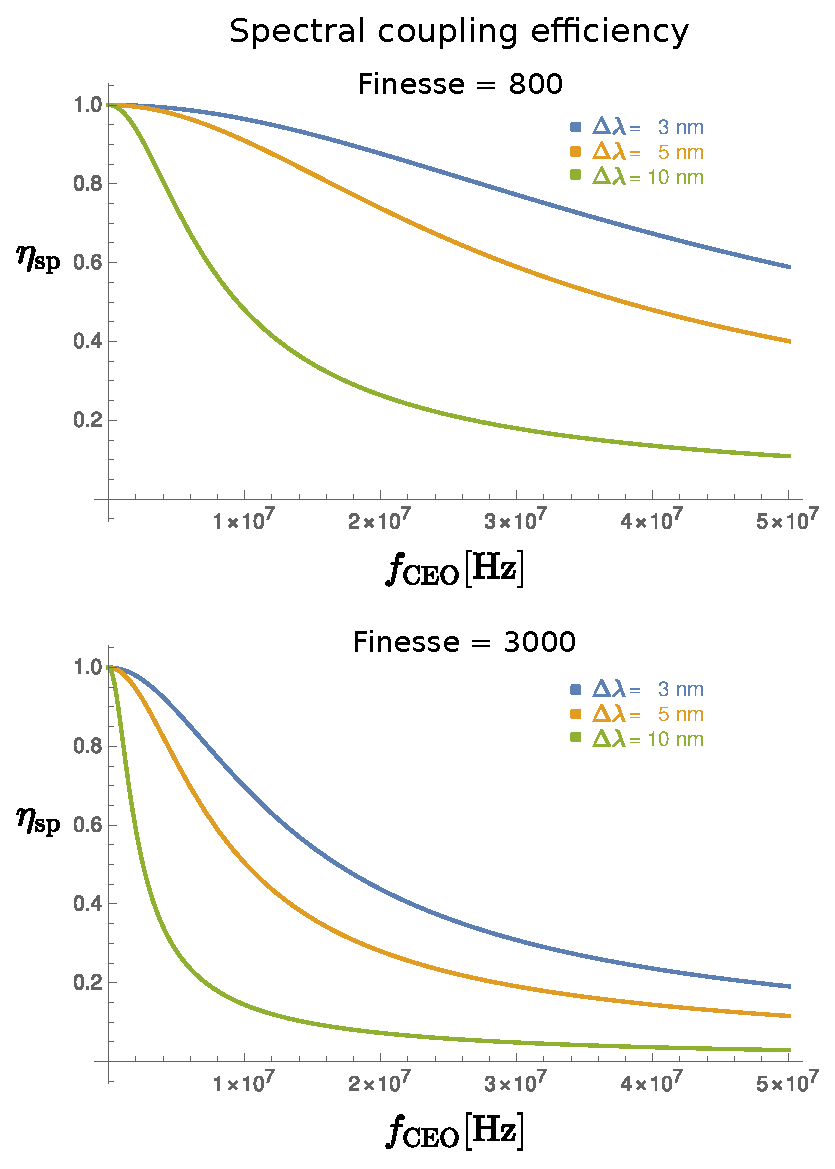
\includegraphics[width=0.9\linewidth]{images/spectraleta.eps}
	\caption{Spectral coupling efficiency as a function of the Carrier-Envelope-Offset frequency $f_\mathrm{CEO}$. The two plots refer to cavities with different Finesse: 800 for the top one and 3000 for the bottom one. The greater the Finesse, the greater the effect on the efficiency.}
	\label{fig:spectraleta}
\end{figure}

\subsubsection{Effect of the mirror dispersion}
When a laser beam reflects on a mirror it experiences a small phase shift $\phi(\lambda)$ caused by the fact that the penetration length is non-zero. This phase shift is different for each wavelength and it changes the effective length of the cavity according to
\begin{align}
	L_\mathrm{eff}(\lambda) = L + \frac{\lambda \phi(\lambda)}{2\pi}
\end{align}	
where $L$ is the length of the cavity while $L_\mathrm{eff}$ the effective length.
We can write the frequencies of the modes $\nu_m$ in a cavity $L_\mathrm{eff}(\lambda)$ long, each mode will see a different cavity length:
\begin{align}
	\nu_{m} = \frac{c}{L} \left( m_0 + \delta m - \frac{\phi(\lambda_{\delta m})}{2\pi} \right)
\end{align}
where as before we have $m = m_0 +\delta m$. If we expand $\phi(\lambda)$ to second order we get:
\begin{align}
	\nu_{m} = \frac{c}{L} \left( m_0 + \delta m -\frac{\phi_0}{2\pi} -\frac{1}{2\pi} \frac{\partial\phi}{\partial\lambda} \delta\lambda - \frac{1}{4\pi} \frac{\partial^2\phi}{\partial\lambda^2} \delta\lambda^2  \right)
\end{align}

Since $\delta\lambda \propto \delta m$, the first order term simply changes the spacing between the cavity resonant frequency by a fixed amount, and can be corrected by changing $L$. The second order term changes instead the spacing between the modes by a different amount for each $m$, introducing again a mismatch between the cavity resonant frequencies and the laser modes. The second order term can be estimated using dielectric mirror theory \parencite{Garmire2003} to
\begin{align}
	\frac{\partial^2\phi}{\partial\lambda^2} = -2.084\times 10^{-5}\,\mathrm{nm}^{-2}
\end{align}
for TiO$_2$-SiO$_2$ mirrors. A plot of the effect of the mirror dispersion on the coupling efficiency is shown in Fig \ref{fig:dispersion}, we can see that for our current Finesse a spectrum of width $\Delta\lambda = 3\,$nm is sufficient while for the final cavity the spectrum must be narrower. The mirror dispersion effect on the coupling efficiency cannot be compensated (as opposed to that given by the $f_\mathrm{CEO}$) and so constitutes a limiting factor on the spectrum that can be coupled in the final Fabry-Perot cavity.
\begin{figure}
	\centering
	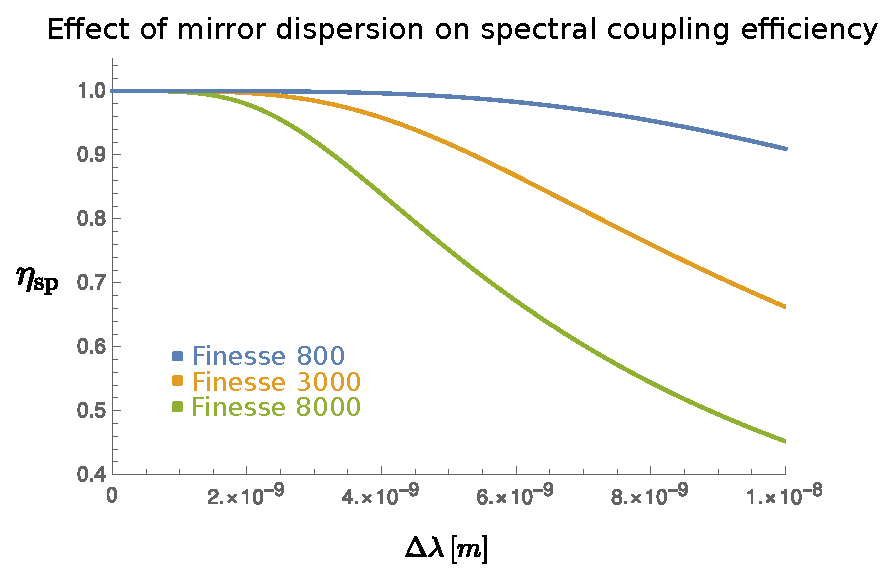
\includegraphics[width=0.9\linewidth]{images/dispersion.eps}
	\caption{Effect of the mirror dispersion on the spectral coupling efficiency. The effect is greater for higher Finesse. The only way to mitigate the effect is to reduce the input radiation spectral width.}
	\label{fig:dispersion}
\end{figure}

\subsection{Thermal effects and the compensation method}
\begin{figure}
	\centering
	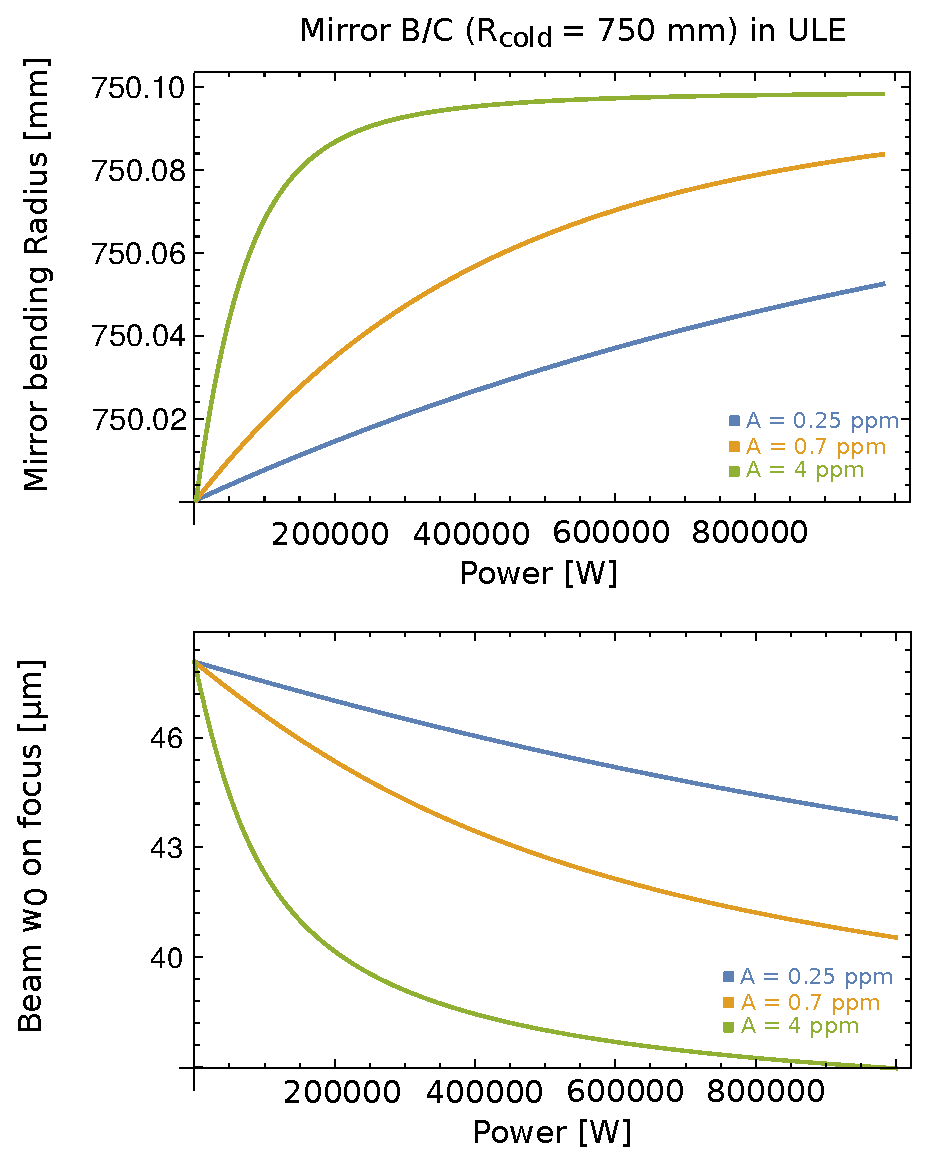
\includegraphics[width=0.9\linewidth]{images/mirrordef.eps}
	\caption{Top: radius of curvature of mirrors B and C versus power. The substrate material of choice for BriXS is ULE (Ultra Low Expansion) for its reduced thermal deformation. Bottom: waist size versus power, to compensate for the waist size change the distance between mirrors B and C has to be corrected. Different colors refer to different mirror absorption.}
	\label{fig:mirrordef}
\end{figure}
\begin{figure}
	\centering
	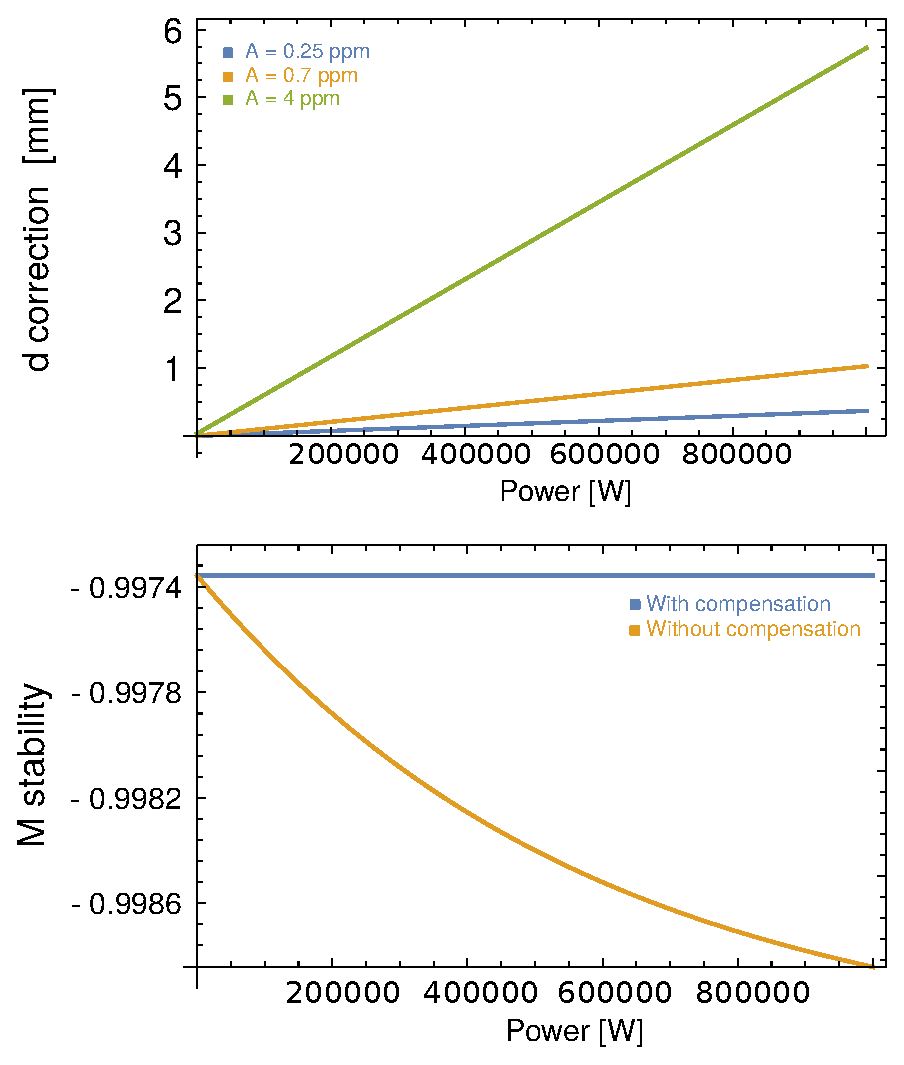
\includegraphics[width=0.9\linewidth]{images/compensation.eps}
	\caption{Top: correction length for the curved mirror distance B-C as a function of cavity internal power. Bottom: stability parameter $m_V$ as a function of cavity internal power, without compensation the stability parameter goes towards the stability edge $m=-1$, by implementing the correction from the top plot the stability parameter is kept constant.}
	\label{fig:compensation}
\end{figure}
\begin{figure}
	\centering
	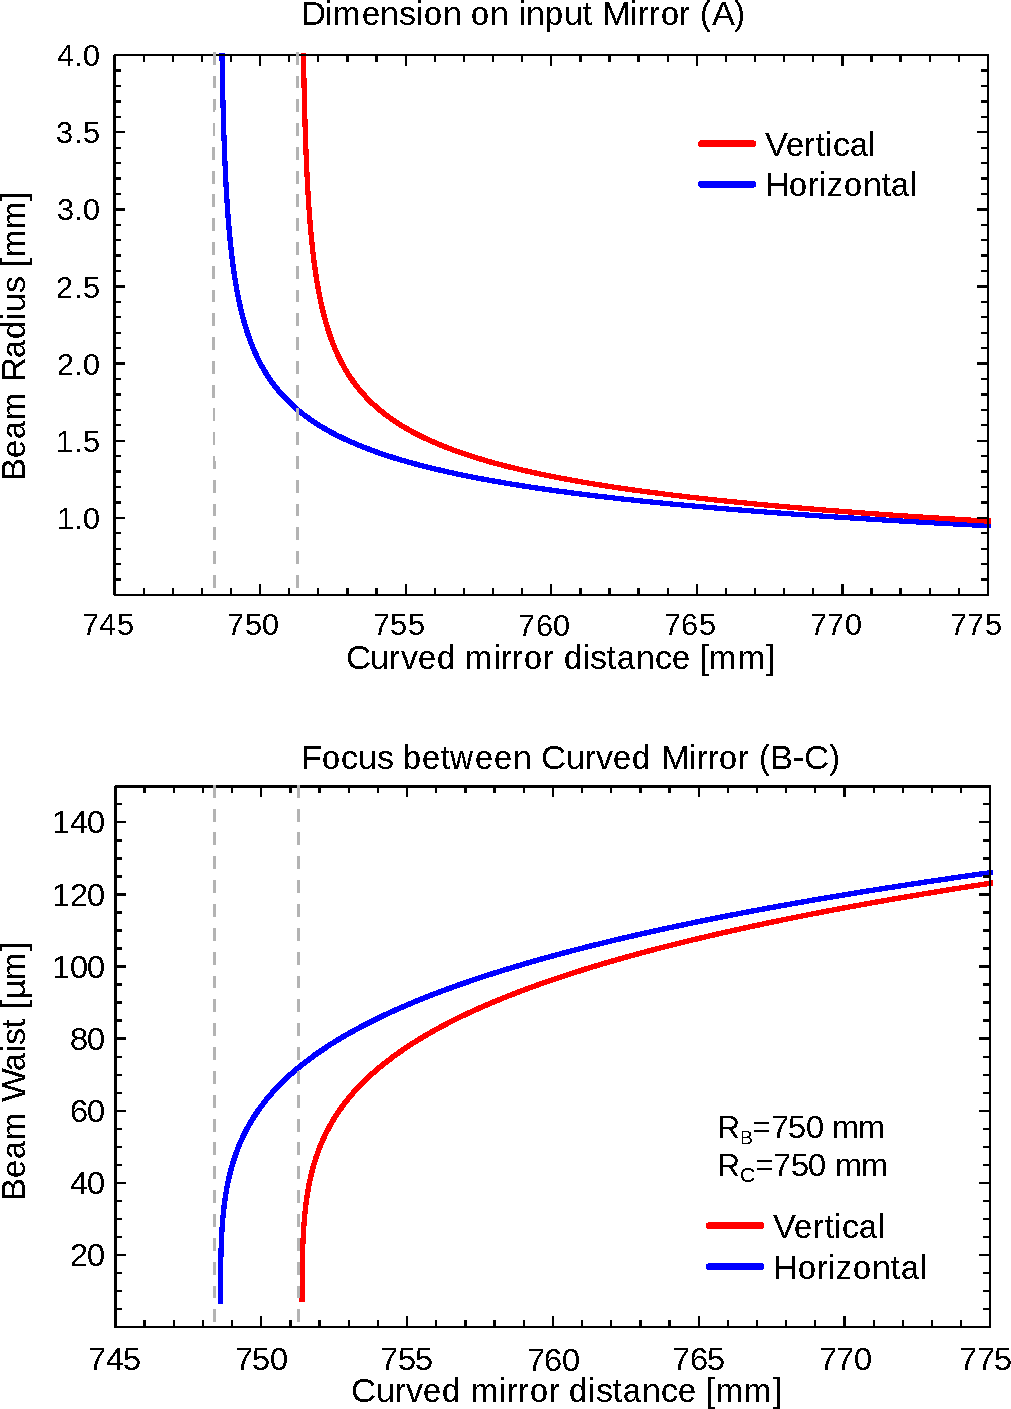
\includegraphics[width=0.9\linewidth]{images/spotdim.pdf}
	\caption{Top: Spot size on the input mirror A, as the cavity becomes near-confocal the spot size increases, diminishing the thermal deformation. Bottom: Waist size in the cavity focus, in the near-confocal configuration the size vanishes. The difference between the vertical and horizontal size is a consequence of the astigmatism of the curved mirrors, which have a different effective radius in the two directions.}
	\label{fig:spotdim}
\end{figure}

In a high-gain Fabry-Perot cavity the internal power can cause the mirrors to change shape because of the thermal deformation of the mirror surface. In particular a mirror heated by a gaussian beam gains an additional curvature given by \parencite{Winkler1991}:
\begin{align}
\frac{1}{R_t} = -\gamma \frac{a}{k} \frac{P}{2\pi w^2}
\end{align}
where $k$ is the thermal conductivity, $a$ the expansion coefficient, $\gamma$ the mirror absorption and $P$ the optical power.
The total radius can then be found as:
\begin{align}
	\frac{1}{R_\mathrm{warm}} = \frac{1}{R_\mathrm{cold}} +  \frac{1}{R_t}
\end{align}
The waist size and the spot size at the mirrors surface both depend on the radius of curvature, this means that they also depend on the internal power of the cavity. In \ref{fig:mirrordef} we can see the relation between the waist size and the internal optical power: as the radius of curvature gets bigger so does the cavity waist. The size depends also on the curved mirror separation (for our cavity the relation is shown in Fig \ref{fig:spotdim}): it is then possible to calculate a mirror separation B-C that keeps the cavity focus at the same size for every power. Since the cavity must maintain its length to couple with the laser, we simultaneously have to change the position of mirror D. This ``compensation method'' can be realized by mounting the mirrors on piezoelectric driven sleds, an essential requirement is that the cavity remains stabilized during the movement.

\subsubsection{Degenerate mode coupling}

It is known that in a high-Finesse optical resonator non-ideal effects like mirror roughness and non-infinite mirror size can cause unwanted losses through
a process known as resonant mode coupling \parencite{Klaassen2005,Kleckner2010,Benedikter2015}. When two cavity modes have the same resonant frequency, energy transfer can occur between them because of cavity non-idealities, such as mirror roughness or finite size. This can lead to increased losses as the coupling between the cavity fundamental mode and the external oscillator mode is reduced. Frequency degeneracy can occur for particular cavity geometries (which translates to particular $m_V$ and $m_H$ parameters), since thermal expansion can change the stability parameters mode coupling can be a problem for BriXS cavities.
\begin{figure}
	\centering
	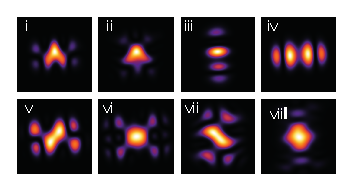
\includegraphics[width=0.9\linewidth]{images/modemixing.eps}
	\caption{Possible cavity fundamental eigenmodes when resonant mode coupling occurs, observed by \parencite{Benedikter2015} by varying the cavity length. The fundamental mode consists of a superposition of the $HG_{00}$ with a higher order mode, such as the $HG_{14}$ in figure $\boldsymbol{i}$.  }
	\label{fig:modemixing}
\end{figure}

To account for mirror surface imperfections and finite size, we introduce the ``mode-mixing operator'' \parencite{Kleckner2010}:
\begin{align}
\mathrm{M}=\exp(ikL)\mathrm{A}\times{B}
\end{align}
where A and B represent the effect of mirrors on the mode (and may be more than two,
our cavity has four mirrors).
Cavity modes $\ket{\psi_\mathrm{i}}$ (we use Dirac notation) satisfy:
\begin{equation}
\gamma_\mathrm{i}\ket{\psi_\mathrm{i}} = \mathrm{M}\ket{\psi_\mathrm{i}}
\end{equation}
where $\gamma_\mathrm{i}$ must be real for the mode to resonate and $D=1-|\gamma_\mathrm{i}|^2$ represents the power loss after a round trip. The ``ground state'' of the cavity is the mode with minimum power loss.
We can express the mirror operators A and B and the mode-mixing operator M in the Hermite-Gauss basis $\{\ket{\phi_{nm}}\}$:
\begin{equation}
\label{A}
\mathrm{A}_{nm,st} = \frac{1}{T}\int dt\iint_S dxdy\ \phi_{nm}\phi_{st}^*e^{-2ik\Delta_a(x,y)}
\end{equation}
where $\Delta_a(x,y)$ is the deviation of the mirror from a plane given by the mirror roughness (the factor 2 is needed to account both for the incident and the reflected beam) and $\phi_i$ are the Hermite-Gauss modes (see \ref{eq:HG}). The spatial integral is taken over the surface of the mirror and the temporal integral averages the value over multiple round trips. This is very important because then $\mathrm{A_{nm,st}}$ is non-zero only if the two modes share the same frequency $\nu$. In the case of perfect mirrors A is the identity matrix and the cavity eigenmodes correspond to the Hermite-Gauss set, with $HG_{00}$ as fundamental mode. If $\Delta_{a,b}(x,y) \ne 0$ A and M are not diagonal and energy transfer occurs between the Hermite-Gauss modes. The new eigenmodes of the cavity are given by diagonalizing M and will in general be superpositions of the HG modes (see Fig \ref{fig:modemixing}). When this happens the coupling between the external ($HG_{00}$) mode and the cavity eigenmode is reduced as their overlap integral becomes smaller.  We note that the overlap integral \ref{A} of a $HG_{nm}$ mode with the $HG_{00}$ becomes smaller the greater $n+m$ is, so we expect higher order modes to contribute less to mode coupling.

In a cavity affected by mode coupling the internal power undergoes periodical fluctuations: firstly thermal deformations introduce losses through mode coupling, these losses reduce the internal power, the temperature of the mirror decreases restoring their shape, now the power can increase again and the process restarts.

The ``compensation method'' used to change the cavity waist size can also be employed to avoid cavity modes to become degenerate by controlling the $m$ parameters of the cavity.